% Communication job: show validation, correction, and convergence to output.
% Primary grammar: decision workflow with one corrective branch.
% Target geometry: single-column figure, natural width approximately 8.5 cm or less.
% Semantic status: schematic.
% Compile with: pdflatex decision-workflow.tex
\documentclass[tikz,border=2mm,10pt]{standalone}

\usetikzlibrary{arrows.meta,positioning,shapes.geometric,calc}

\definecolor{figdark}{gray}{0.25}
\definecolor{figlight}{gray}{0.85}

\tikzset{
  terminal/.style={
    rectangle, draw=figdark, fill=white,
    minimum width=1.05cm, minimum height=0.65cm,
    align=center, inner sep=3pt
  },
  block/.style={
    rectangle, draw=figdark, fill=figlight,
    minimum width=1.35cm, minimum height=0.75cm,
    align=center, inner sep=3pt
  },
  decision/.style={
    diamond, draw=figdark, fill=figlight,
    aspect=1.6, minimum width=1.35cm,
    minimum height=0.95cm, align=center, inner sep=1pt
  },
  arrow/.style={->, >={Stealth[length=1.8mm]}, thick, draw=figdark},
  edgelabel/.style={font=\footnotesize, fill=white, inner sep=1pt}
}

\begin{document}
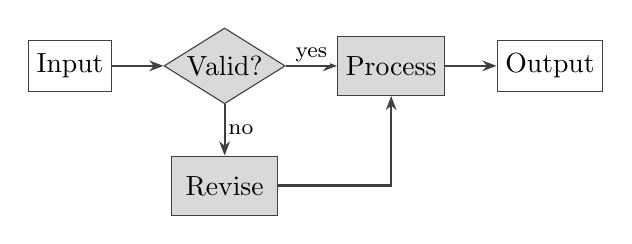
\begin{tikzpicture}[node distance=0.55cm and 0.65cm]
  \node[terminal] (input) {Input};
  \node[decision, right=of input] (check) {Valid?};
  \node[block, right=of check] (process) {Process};
  \node[terminal, right=of process] (output) {Output};
  \node[block, below=0.65cm of check] (revise) {Revise};

  \draw[arrow] (input) -- (check);
  \draw[arrow] (check) -- node[edgelabel, above] {yes} (process);
  \draw[arrow] (process) -- (output);
  \draw[arrow] (check.south) -- node[edgelabel, right] {no} (revise.north);
  \draw[arrow] (revise.east) -| (process.south);
\end{tikzpicture}
\end{document}
